
\chapter[Classificação e Registro do Produto]{Classificação e Registro do Produto}

Produtos biomédicos para serem regularizados devem passar por diversas avaliações e classificações. Uma das principais classificações feitas em um produto biomédico diz respeito ao risco em que o paciente está submetido ao usá-lo. A resolução RDC nº 185/2001 traz em seus anexos regras para se classificar um produto biomédico quanto ao risco. A Seção 1.1. destaca essas regras e a classificação do posicionador de lentes quanto ao risco.


\section[Regularização de Equipamentos Médicos na Anvisa]{Regularização de Equipamentos Médicos na Anvisa}

Equipamentos de uso em saúde que possuam finalidade médica, odontológica, laboratorial ou fisioterápica, utilizados em diagnóstico, terapia, reabilitação, monitoração de seres humanos ou com finalidade de embelezamento e estética estão sob-regime de Vigilância Sanitária (ANVISA, 2001).
	
A resolução RDC nº 185/2001 da Anvisa fornece orientações sobre o registro, cadastramento, alteração, revalidação e cancelado do registro de produtos médicos (ANVISA, 2001). Segundo o Art. 12 da Lei 6.369/1976, nenhum produto que está sujeito à vigilância sanitária, inclusive os importados, poderá ser industrializado, exposto à venda ou entregue ao consumo antes de registrado no Ministério da Saúde. A resolução também é aplicada a equipamentos, aparelhos, materiais, artigos ou sistemas de uso ou aplicação em educação física embelezamento ou correção estética.

Os produtos médicos sujeitos à vigilância sanitária são enquadrados segundo o risco que representam à saúde do consumidor, paciente, operador ou terceiros envolvidos em Classes, as quais variam entre I a IV. A Classe I representa os produtos de baixo risco. A Classe II engloba os produtos de médio risco. A Classe III é usada para classificar os produtos como de alto risco. Por fim, a Classe IV representa os produtos de máximo risco. Para se classificar os produtos, devem ser aplicadas as regras de classificação, descritas na tabela 3.

\vspace{\onelineskip} 
 \vspace{\onelineskip}
\vspace{\onelineskip} 
 \vspace{\onelineskip}
\vspace{\onelineskip} 
 \vspace{\onelineskip}
\vspace{\onelineskip} 
 \vspace{\onelineskip}
\vspace{\onelineskip} 

% Please add the following required packages to your document preamble:
% \usepackage{multirow}
{
\center
{
\scriptsize
\begin{longtable}{|c|c|l|}
\hline
\textbf{Tipo do Produto}          & \textbf{Regra} & \multicolumn{1}{c|}{\textbf{Descrição}}                                                                                                                                                                                                                                                                                                                                                                                                                                                                                                                                                                                                                                                                                                                                                                                                                                                                                                                                                                                                                                                                                                \\ \hline
\multirow{4}{*}{Não invasivos}    & 1              & \begin{tabular}[c]{@{}l@{}}Todos os produtos médicos não invasivos estão na\\   classe I, exceto aqueles aos quais se aplicam as regras 2, 3 e 4.\end{tabular}                                                                                                                                                                                                                                                                                                                                                                                                                                                                                                                                                                                                                                                                                                                                                                                                                                                                                                                                                                         \\ \cline{2-3} 
                                  & 2              & \begin{tabular}[c]{@{}l@{}}Todos os produtos\\ médicos não-invasivos destinados ao armazenamento ou condução de sangue,\\ fluidos ou tecidos corporais, líquidos ou gases destinados a perfusão,\\ administração ou introdução no corpo, estão na Classe II:,\\ a) se puderem ser\\ conectados a um produto médico ativo da Classe II ou de uma Classe superior; e,\\ b) se forem destinados à condução, armazenamento ou\\ transporte de sangue ou de outros fluidos corporais ou armazenamento de órgãos,\\ partes de órgãos ou tecidos do corpo.\end{tabular}                                                                                                                                                                                                                                                                                                                                                                                                                                                                                                                                                                       \\ \cline{2-3} 
                                  & 3              & \begin{tabular}[c]{@{}l@{}}Todos os produtos médicos não-invasivos\\ destinados a modificar a composição química ou biológica do sangue, de outros\\ fluidos corporais ou de outros líquidos destinados a introdução no corpo, estão\\ na Classe III, exceto se o tratamento consiste de filtração, centrifugação ou\\ trocas de gases ou de calor, nestes casos pertencem à Classe II.\end{tabular}                                                                                                                                                                                                                                                                                                                                                                                                                                                                                                                                                                                                                                                                                                                                   \\ \cline{2-3} 
                                  & 4              & \begin{tabular}[c]{@{}l@{}}Todos os produtos\\ médicos não-invasivos que entrem em contato com a pele lesada:,\\ a) enquadram-se na\\ Classe I se estão destinados a ser usados como barreira mecânica, para\\ compressão ou para absorção de exsudados;\\ b) enquadram-se na\\ Classe III se estão destinados a ser usados principalmente em feridas que\\ tenham produzido ruptura da derme e que somente podem cicatrizar por segunda\\ intenção; e,\\ c) enquadram-se na Classe II em todos outros casos,\\ incluindo os produtos médicos destinados principalmente a atuar no\\ micro-entorno de uma ferida\end{tabular}                                                                                                                                                                                                                                                                                                                                                                                                                                                                                                          \\ \hline
\multirow{4}{*}{Invasivos}        & 5              & \begin{tabular}[c]{@{}l@{}}Todos os produtos\\ médicos invasivos aplicáveis aos orifícios do corpo, exceto os produtos médicos\\ invasivos cirurgicamente, que não sejam destinados à conexão com um produto\\ médico ativo:,\\ a) enquadram-se na\\ Classe I se forem destinados a uso transitório;\\ b) enquadram-se na\\ Classe II se forem destinados a uso de curto prazo, exceto se forem usados na\\ cavidade oral até a faringe, no conduto auditivo externo até o tímpano ou na\\ cavidade nasal, nestes casos enquadram-se na Classe I; e,\\ c) enquadram-se na\\ Classe III se forem destinados a uso de longo prazo, exceto se forem usados na cavidade\\ oral até a faringe, no conduto auditivo externo até o tímpano ou na cavidade\\ nasal e não forem absorvíveis pela membrana mucosa, nestes casos enquadram-se\\ na Classe II.\\ Todos os produtos médicos invasivos aplicáveis aos\\ orifícios do corpo, exceto os produtos médicos invasivos cirurgicamente, que se\\ destinem a conexão com um produto médico ativo da Classe II ou de uma Classe\\ superior, enquadram-se na Classe II.\end{tabular}           \\ \cline{2-3} 
                                  & 6              & \begin{tabular}[c]{@{}l@{}}Todos os produtos\\ médicos invasivos cirurgicamente de uso transitório enquadram-se na Classe II,\\ exceto se:\\ a) se destinarem\\ especificamente ao diagnóstico, monitoração ou correção de disfunção cardíaca\\ ou do sistema circulatório central, através de contato direto com estas partes\\ do corpo, nestes casos enquadra-se na Classe IV;\\ b) forem\\ instrumentos cirúrgicos reutilizáveis, nestes casos enquadram-se na Classe I;\\ c) se destinarem a\\ fornecer energia na forma de radiações ionizantes, caso em que se enquadram na\\ Classe III;\\ d) se destinarem a\\ exercer efeito biológico ou a ser totalmente ou em grande parte absorvidos,\\ nestes casos pertencem à Classe III;\\ e) se destinarem a administração de medicamentos por\\ meio de um sistema de infusão, quando realizado de forma potencialmente\\ perigosa, considerando o modo de aplicação, neste caso enquadram-se na Classe\\ III.\end{tabular}                                                                                                                                                        \\ \cline{2-3} 
                                  & 7              & \begin{tabular}[c]{@{}l@{}}Todos os produtos\\ médicos invasivos cirurgicamente de uso em curto prazo enquadram-se na Classe\\ II, exceto no caso em que se destinem:\\ a) especificamente\\ ao diagnóstico, monitoração ou correção de disfunção cardíaca ou do sistema\\ circulatório central, através de contato direto com estas partes do corpo,\\ nestes casos enquadram-se na Classe IV; ou,\\ b) especificamente\\ a ser utilizados em contato direto com o sistema nervoso central, neste caso\\ enquadram-se na Classe IV; ou,\\ c) a administrar\\ energia na forma de radiações ionizantes, neste caso enquadram-se na Classe\\ III; ou,\\ d) a exercer\\ efeito biológico ou a ser totalmente ou em grande parte absorvidos, nestes\\ casos enquadram-se na Classe IV; ou,\\ e) a sofrer alterações químicas no organismo ou para\\ administrar medicamentos, excluindo-se os produtos médicos destinados a ser\\ colocados dentro dos dentes, neste caso pertencem à Classe III.\end{tabular}                                                                                                                            \\ \cline{2-3} 
                                  & 8              & \begin{tabular}[c]{@{}l@{}}Todos os produtos\\ médicos implantáveis e os produtos médicos invasivos cirurgicamente de uso em\\ longo prazo enquadram-se na Classe III, exceto no caso de se destinarem:\\ a) a ser colocados\\ nos dentes, neste caso pertencem à Classe II;\\ b) a ser\\ utilizados em contato direto com o coração, sistema circulatório central ou\\ sistema nervoso central, neste caso pertencem á Classe IV;\\ c) a produzir um\\ efeito biológico ou a ser absorbidos, totalmente ou em grande parte, neste caso\\ pertencem á Classe IV;\\ d) a sofrer uma transformação química no corpo ou\\ administrar medicamentos, exceto se forem destinados a ser colocados nos\\ dentes, nestes casos pertencem á Classe IV.\end{tabular}                                                                                                                                                                                                                                                                                                                                                                             \\ \hline
\multirow{4}{*}{Médicos Ativos}   & 9              & \begin{tabular}[c]{@{}l@{}}Todos os produtos\\ médicos ativos para terapia destinados a administrar ou trocar energia\\ enquadram-se na Classe II, exceto se suas características são tais que possam\\ administrar ou trocar energia com o corpo humano de forma potencialmente\\ perigosa, considerando-se a natureza, a densidade e o local de aplicação da\\ energia, neste caso enquadram-se na Classe III;\\ Todos os produtos ativos destinados a controlar ou\\ monitorar o funcionamento de produtos médicos ativos para terapia enquadrados\\ na Classe III ou destinados a influenciar diretamente no funcionamento destes\\ produtos, enquadram-se na Classe III.\end{tabular}                                                                                                                                                                                                                                                                                                                                                                                                                                             \\ \cline{2-3} 
                                  & 10             & \begin{tabular}[c]{@{}l@{}}Os produtos\\ médicos ativos para diagnóstico ou monitoração estão na Classe II:\\ a) caso\\ destinem-se a administrar energia a ser absorvida pelo corpo humano, exceto os\\ produtos médicos cuja função seja iluminar o corpo do paciente no espectro\\ visível;\\ b) caso\\ destinem-se a produzir imagens “in-vivo” da distribuição de radiofármacos;\\ c) caso destinem-se\\ ao diagnóstico direto ou a monitoração de processos fisiológicos vitais, a não\\ ser que se destinem especificamente à monitoração de parâmetros fisiológicos\\ vitais, cujas variações possam resultar em risco imediato à vida do paciente,\\ tais como variações no funcionamento cardíaco, da respiração ou da atividade do\\ sistema nervoso central, neste caso pertencem à Classe III.\\ Os produtos médicos ativos destinados a emitir\\ radiações ionizantes, para fins radiodiagnósticos ou radioterapêuticos,\\ incluindo os produtos destinados a controlar ou monitorar tais produtos médicos\\ ou que influenciam diretamente no funcionamento destes produtos, enquadram-se\\ na Classe III.\end{tabular} \\ \cline{2-3} 
                                  & 11             & \begin{tabular}[c]{@{}l@{}}Todos os produtos médicos ativos destinados a\\ administrar medicamentos, fluidos corporais ou outras substâncias do organismo\\ ou a extraí-los deste, enquadram-se na Classe II, a não ser que isto seja\\ realizado de forma potencialmente perigosa, considerando a natureza das\\ substâncias, a parte do corpo envolvida e o modo de aplicação, neste caso\\ enquadram-se na Classe III.\end{tabular}                                                                                                                                                                                                                                                                                                                                                                                                                                                                                                                                                                                                                                                                                                 \\ \cline{2-3} 
                                  & 12             & \begin{tabular}[c]{@{}l@{}}Todos os demais produtos médicos ativos\\ enquadram-se na Classe I.\end{tabular}                                                                                                                                                                                                                                                                                                                                                                                                                                                                                                                                                                                                                                                                                                                                                                                                                                                                                                                                                                                                                            \\ \hline
\multirow{6}{*}{Regras Especiais} & 13             & \begin{tabular}[c]{@{}l@{}}Todos os produtos médicos que incorporem como\\ parte integrante uma substância, que utilizada separadamente possa ser\\ considerada um medicamento, e que possa exercer sobre o corpo humano uma ação\\ complementar à destes produtos, enquadram-se na Classe IV.\end{tabular}                                                                                                                                                                                                                                                                                                                                                                                                                                                                                                                                                                                                                                                                                                                                                                                                                            \\ \cline{2-3} 
                                  & 14             & \begin{tabular}[c]{@{}l@{}}Todos os produtos médicos utilizados na\\ contracepção ou para prevenção da transmissão de doenças sexualmente transmissíveis\\ enquadram-se na Classe III, a não ser que se trate de produtos médicos\\ implantáveis ou de produtos médicos invasivos destinados a uso de longo prazo,\\ neste caso pertencem á classe IV.\end{tabular}                                                                                                                                                                                                                                                                                                                                                                                                                                                                                                                                                                                                                                                                                                                                                                    \\ \cline{2-3} 
                                  & 15             & \begin{tabular}[c]{@{}l@{}}Todos os produtos\\ médicos destinados especificamente a desinfetar, limpar, lavar e, se\\ necessário, hidratar lentes de contato, enquadram-se na Classe III.\\ Todos os produtos\\ médicos destinados especificamente a desinfetar outros produtos médicos,\\ enquadram-se na Classe II.\\ Esta regra não se aplica aos produtos destinados à\\ limpeza de produtos médicos, que não sejam lentes de contato, por meio de ação\\ física.\end{tabular}                                                                                                                                                                                                                                                                                                                                                                                                                                                                                                                                                                                                                                                     \\ \cline{2-3} 
                                  & 16             & \begin{tabular}[c]{@{}l@{}}Os produtos médicos não-ativos destinados\\ especificamente para o registro de imagens radiográficas para diagnóstico,\\ enquadram-se na Classe II.\end{tabular}                                                                                                                                                                                                                                                                                                                                                                                                                                                                                                                                                                                                                                                                                                                                                                                                                                                                                                                                            \\ \cline{2-3} 
                                  & 17             & \begin{tabular}[c]{@{}l@{}}Todos os produtos médicos que utilizam tecidos\\ de origem animal ou seus derivados tornados inertes enquadram-se na Classe IV,\\ exceto quando tais produtos estejam destinados unicamente a entrar em contato\\ com a pele intacta.\end{tabular}                                                                                                                                                                                                                                                                                                                                                                                                                                                                                                                                                                                                                                                                                                                                                                                                                                                          \\ \cline{2-3} 
                                  & 18             & \begin{tabular}[c]{@{}l@{}}Não obstante o disposto nas outras regras, as\\ bolsas de sangue enquadram-se na enquadram-se na Classe III.\end{tabular}                                                                                                                                                                                                                                                                                                                                                                                                                                                                                                                                                                                                                                                                                                                                                                                                                                                                                                                                                                                   \\ \hline
\caption{Regras de Classificação de Produtos Médicos - Fonte: Resolução RDC nº 185/2001 da Anvisa.}
\end{longtable}
}
}


Considerando o posicionador de lentes de contato, cuja função é a de inserir e retirar lentes de contato do olho humano, de forma invasiva, classifica-se o produto como invasivo. Assim, as regras que são aplicáveis a este produto se resumem nas expostas na tabela 3.  Conforme a regra 5, “todos os produtos médicos invasivos aplicáveis aos orifícios do corpo, exceto os produtos médicos invasivos cirurgicamente, que se destinem a conexão com um produto médico ativo da Classe II ou de uma Classe superior, enquadram-se na Classe II”. Considerando que o posicionador de lentes é um produto médico ativo por depender de fonte de energia elétrica e que insere e extrai um objeto em um orifício do olho, conforme a regra 5, o posicionador de lente é classificado como de Classe II.

\section[Processo de Registro do Produto na Anvisa]{Processo de Registro do Produto na Anvisa}

Segundo a Resolução RDC nº 185/2001 da Anvisa, somente estão isentos de registro os produtos médicos que:
\begin{itemize}
\item São submetidos à pesquisa clínica, estando proibida sua comercialização e/ou uso para outros fins;
\item Compõe novas apresentações constituídas de um conjunto de produtos médicos registrados e em suas embalagens individuais de apresentação íntegras; e
\item São produzidos para integrar um produto médico de sua fabricação já registrado e cujo relatório técnico deste produto contenha informações deste novo acessório.
\end{itemize}

Conforme essas regras, enquanto o posicionador de lentes se encontrar em fase de pesquisa clínica, não será necessário o seu registro. Após a fase de pesquisa e comprovação de funcionamento, para que o posicionador de lentes possa ser comercializado, deverá ser respeitado o processo de registro de produtos na Anvisa.

De acordo com a RDC º 185/2001 da Anvisa, as atividades expostas na tabela 4 são necessárias para registro de um produto na Anvisa:

\begin{table}[h]
\center
\footnotesize
\begin{tabular}{|p{3.5cm}|p{4.5cm}|p{8cm}|}
\hline
\textbf{Atividade}                 & \textbf{Descrição/Análise}                                                                                                   & \multicolumn{1}{c|}{\textbf{Análise}}                                                                                                                                                                                                                                                                                                           \\ \hline
Identificação Sanitária do Produto & \begin{tabular}[c]{@{}c@{}}Tem o objetivo de identificar \\  a necessidade de identificação \\ sanitária do produto.\end{tabular} & \begin{tabular}[c]{@{}l@{}}Por se tratar de um equipamento médico, o\\ posicionador de lentes deverá passar \\  por identificação sanitária, ou seja, está\\ sujeito à vigilância sanitária.\end{tabular}                                                                                                                                           \\ \hline
Documentação                       & \begin{tabular}[c]{@{}c@{}}Visa o preenchimento do \\ formulário de registro\\ do produto.\end{tabular}                         & \begin{tabular}[c]{@{}l@{}}Preenchimento do formulário, cujos itens estão\\ especificados na Resolução RDC 185/2001,  \\ deverá ser feito para registro do\\ posicionador de lentes.\end{tabular}                                                                                                                                                   \\ \hline
Identificação de Família           & \begin{tabular}[c]{@{}c@{}}Visa identificar se o produto \\ é único ou pertencente \\ a uma família de produtos.\end{tabular}    & \begin{tabular}[c]{@{}l@{}}Por se tratar de um produto novo, o posicionador\\ de lentes é considerado um produto único. \\ Dada essa classificação, deverá ser\\ elaborado rótulo, instruções de uso \\ e informações gerais para disponibilização\\ em meio eletrônico.\end{tabular}                                                                 \\ \hline
Enquadramento Sanitário do Produto & \begin{tabular}[c]{@{}c@{}}Visa identificar se o produto \\ está sujeito ao\\ registro sanitário.\end{tabular}                  & \begin{tabular}[c]{@{}l@{}}Na fase de elaboração e de testes clínicos, o\\ posicionador de lentes não estará sujeito ao registro \\ sanitário. Para comercialização e uso, o produto \\ deverá passar pela submissão para registro,\\ devendo ser paga uma taxa de vigilância sanitária \\ e elaborado um relatório\\ técnico do produto.\end{tabular} \\ \hline
Regulamentação Técnica             & \begin{tabular}[c]{@{}c@{}}Visa identificar se o produto \\ está ou não sujeito \\ à certificação\end{tabular}                   & \begin{tabular}[c]{@{}l@{}}Por ser um produto que coloca em risco à saúde\\ do consumidor, deverá ser obtida certificação \\ compulsória para comercialização\\ do posicionador de lentes.\end{tabular}                                                                                                                                            \\ \hline
Interessado                        & \begin{tabular}[c]{@{}c@{}}Visa à identificação do \\ interessado  no registro \\ do produto.\end{tabular}                        & \begin{tabular}[c]{@{}l@{}}Após testes clínicos, para comercialização do\\ produto deverá haver uma empresa interessada. \\ Poderá ser um fabricante\\ instalado no Brasil ou importador.\end{tabular}                                                                                                                                             \\ \hline
Classificação do  Produto           & \begin{tabular}[c]{@{}c@{}}Visa a classificação do \\  produto em um das\\ classes I a IV\end{tabular}                           & \begin{tabular}[c]{@{}l@{}}Conforme exposto na Seção 1.1 deste documento, o\\ posicionador de lentes é classificado como \\ de Classe II. Após classificação,\\ deverá ser apresentada autorização do fabricante \\ e registro ou certificado de livre\\ comércio.\end{tabular}                                                                       \\ \hline
\end{tabular}
\caption{Atividades para Registro de Produtos na Anvisa - Fonte: Resolução RDC nº 185/2001 da Anvisa.}
\end{table}

A Figura \ref{registro} apresenta um diagrama que descreve o processo descrito pela tabela 4.

\begin{figure}[htb]
		\centering
			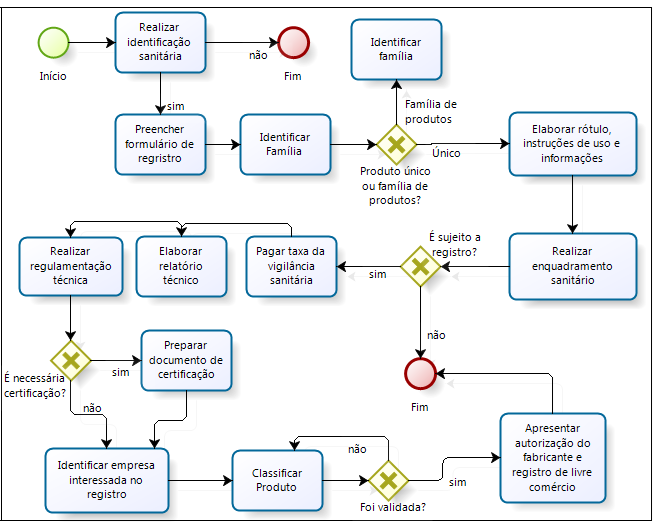
\includegraphics[scale=0.9]{figuras/processoregistro.png}
		\caption{Processo de Registro na Anvisa}
		\label{registro}
\end{figure}


